% Options for packages loaded elsewhere
\PassOptionsToPackage{unicode}{hyperref}
\PassOptionsToPackage{hyphens}{url}
%
\documentclass[
]{article}
\usepackage{lmodern}
\usepackage{amsmath}
\usepackage{ifxetex,ifluatex}
\ifnum 0\ifxetex 1\fi\ifluatex 1\fi=0 % if pdftex
  \usepackage[T1]{fontenc}
  \usepackage[utf8]{inputenc}
  \usepackage{textcomp} % provide euro and other symbols
  \usepackage{amssymb}
\else % if luatex or xetex
  \usepackage{unicode-math}
  \defaultfontfeatures{Scale=MatchLowercase}
  \defaultfontfeatures[\rmfamily]{Ligatures=TeX,Scale=1}
\fi
% Use upquote if available, for straight quotes in verbatim environments
\IfFileExists{upquote.sty}{\usepackage{upquote}}{}
\IfFileExists{microtype.sty}{% use microtype if available
  \usepackage[]{microtype}
  \UseMicrotypeSet[protrusion]{basicmath} % disable protrusion for tt fonts
}{}
\makeatletter
\@ifundefined{KOMAClassName}{% if non-KOMA class
  \IfFileExists{parskip.sty}{%
    \usepackage{parskip}
  }{% else
    \setlength{\parindent}{0pt}
    \setlength{\parskip}{6pt plus 2pt minus 1pt}}
}{% if KOMA class
  \KOMAoptions{parskip=half}}
\makeatother
\usepackage{xcolor}
\IfFileExists{xurl.sty}{\usepackage{xurl}}{} % add URL line breaks if available
\IfFileExists{bookmark.sty}{\usepackage{bookmark}}{\usepackage{hyperref}}
\hypersetup{
  pdftitle={Birthday Problem},
  pdfauthor={coop711},
  hidelinks,
  pdfcreator={LaTeX via pandoc}}
\urlstyle{same} % disable monospaced font for URLs
\usepackage[margin=1in]{geometry}
\usepackage{longtable,booktabs}
\usepackage{calc} % for calculating minipage widths
% Correct order of tables after \paragraph or \subparagraph
\usepackage{etoolbox}
\makeatletter
\patchcmd\longtable{\par}{\if@noskipsec\mbox{}\fi\par}{}{}
\makeatother
% Allow footnotes in longtable head/foot
\IfFileExists{footnotehyper.sty}{\usepackage{footnotehyper}}{\usepackage{footnote}}
\makesavenoteenv{longtable}
\usepackage{graphicx}
\makeatletter
\def\maxwidth{\ifdim\Gin@nat@width>\linewidth\linewidth\else\Gin@nat@width\fi}
\def\maxheight{\ifdim\Gin@nat@height>\textheight\textheight\else\Gin@nat@height\fi}
\makeatother
% Scale images if necessary, so that they will not overflow the page
% margins by default, and it is still possible to overwrite the defaults
% using explicit options in \includegraphics[width, height, ...]{}
\setkeys{Gin}{width=\maxwidth,height=\maxheight,keepaspectratio}
% Set default figure placement to htbp
\makeatletter
\def\fps@figure{htbp}
\makeatother
\setlength{\emergencystretch}{3em} % prevent overfull lines
\providecommand{\tightlist}{%
  \setlength{\itemsep}{0pt}\setlength{\parskip}{0pt}}
\setcounter{secnumdepth}{-\maxdimen} % remove section numbering
\ifluatex
  \usepackage{selnolig}  % disable illegal ligatures
\fi

\title{Birthday Problem}
\author{coop711}
\date{2019-04-29}

\begin{document}
\maketitle

\hypertarget{data}{%
\subsection{Data}\label{data}}

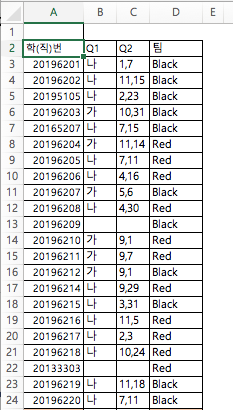
\includegraphics[width=0.33\linewidth]{../pics/birthday_sample_excel}

\hypertarget{uxc0dduxc77c-uxbb38uxc81cuxc758-uxc9c8uxbb38}{%
\subsection{생일 문제의
질문}\label{uxc0dduxc77c-uxbb38uxc81cuxc758-uxc9c8uxbb38}}

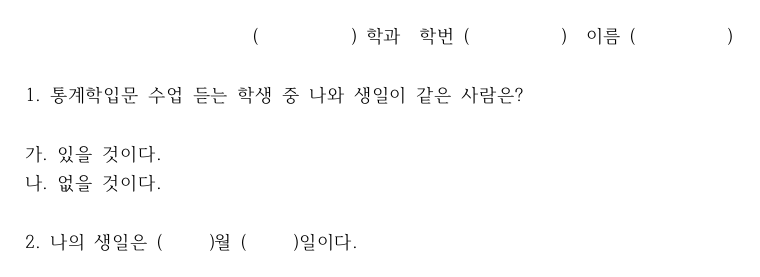
\includegraphics[width=0.75\linewidth]{../pics/birthday_Qs}

\hypertarget{q2.-birthday-problem}{%
\subsubsection{Q2. Birthday Problem}\label{q2.-birthday-problem}}

\hypertarget{uxc0dduxc77cuxc774-uxac19uxc740-uxc0acuxb78cuxc758-uxc218uxd6a8}{%
\paragraph{생일이 같은 사람의
수효}\label{uxc0dduxc77cuxc774-uxac19uxc740-uxc0acuxb78cuxc758-uxc218uxd6a8}}

\begin{longtable}[]{@{}ccc@{}}
\toprule
학번 & 생일 & 그룹\tabularnewline
\midrule
\endhead
20196278 & 01월22일 & Black\tabularnewline
20196283 & 01월22일 & Red\tabularnewline
20196205 & 07월11일 & Red\tabularnewline
20196220 & 07월11일 & Black\tabularnewline
20183940 & 07월12일 & Black\tabularnewline
20196277 & 07월12일 & Red\tabularnewline
20196210 & 09월01일 & Red\tabularnewline
20196212 & 09월01일 & Black\tabularnewline
20196225 & 09월01일 & Black\tabularnewline
20196203 & 10월31일 & Black\tabularnewline
20196285 & 10월31일 & Black\tabularnewline
\bottomrule
\end{longtable}

\hypertarget{uxc5b4uxb290-uxb0a0uxc5d0-uxba87-uxba85uxc529-uxc0dduxc77cuxc774-uxac19uxc740uxac00}{%
\paragraph{어느 날에 몇 명씩 생일이
같은가?}\label{uxc5b4uxb290-uxb0a0uxc5d0-uxba87-uxba85uxc529-uxc0dduxc77cuxc774-uxac19uxc740uxac00}}

\begin{longtable}[]{@{}rrrrrr@{}}
\toprule
01월22일 & 07월11일 & 07월12일 & 09월01일 & 10월31일 & 계\tabularnewline
\midrule
\endhead
2 & 2 & 2 & 3 & 2 & 11\tabularnewline
\bottomrule
\end{longtable}

\hypertarget{uxc0dduxc77cuxc774-uxac19uxc740-uxc0acuxb78cuxc740-uxba87-uxba85-uxc815uxb3c4-uxae30uxb300uxb418uxb294uxac00}{%
\paragraph{생일이 같은 사람은 몇 명 정도
기대되는가?}\label{uxc0dduxc77cuxc774-uxac19uxc740-uxc0acuxb78cuxc740-uxba87-uxba85-uxc815uxb3c4-uxae30uxb300uxb418uxb294uxac00}}

\(N\)을 전체 인원이라 할 때, 기대 인원은
\(N\times\{1- (\frac{364}{365})^{N-1}\}\), 분산은
\(N\times\{1- (\frac{364}{365})^{N-1}\} + N\times(N-1)\times\{1-(\frac{363}{365})^{N-2}\}\)로
계산된다.

무응답이거나 결석한 학생을 제외한 응답 인원 62명에 대하여 기대인원을
계산하면 9.6명, 표준오차는 3.1명으로 계산되어 관찰된 값이 그 범위 근처에
있음을 알 수 있다.

\hypertarget{uxae30uxb300uxac12uxc758-uxacc4uxc0b0}{%
\subparagraph{기대값의
계산}\label{uxae30uxb300uxac12uxc758-uxacc4uxc0b0}}

\begin{verbatim}
## [1] 9.6
\end{verbatim}

\hypertarget{uxd45cuxc900uxc624uxcc28uxc758-uxacc4uxc0b0}{%
\subparagraph{표준오차의
계산}\label{uxd45cuxc900uxc624uxcc28uxc758-uxacc4uxc0b0}}

\begin{verbatim}
## [1] 3.1
\end{verbatim}

\hypertarget{uxd0dcuxc5b4uxb09c-uxb2ecuxc758-uxbd84uxd3ecuxb294}{%
\paragraph{태어난 달의
분포는?}\label{uxd0dcuxc5b4uxb09c-uxb2ecuxc758-uxbd84uxd3ecuxb294}}

\begin{longtable}[]{@{}lrrrrrrrrrrrrr@{}}
\toprule
& 1월 & 2월 & 3월 & 4월 & 5월 & 6월 & 7월 & 8월 & 9월 & 10월 & 11월 &
12월 & 계\tabularnewline
\midrule
\endhead
Red & 3 & 5 & 1 & 4 & 2 & 4 & 1 & 5 & 2 & 3 & 1 & 1 & 32\tabularnewline
Black & 3 & 4 & 2 & 2 & 6 & 2 & 2 & 2 & 2 & 0 & 5 & 0 &
30\tabularnewline
계 & 6 & 9 & 3 & 6 & 8 & 6 & 3 & 7 & 4 & 3 & 6 & 1 & 62\tabularnewline
\bottomrule
\end{longtable}

\hypertarget{uxb79cuxb364uxd654-uxd6a8uxacfc-uxac80uxc99d}{%
\paragraph{랜덤화 효과
검증}\label{uxb79cuxb364uxd654-uxd6a8uxacfc-uxac80uxc99d}}

\begin{longtable}[]{@{}rrr@{}}
\caption{Pearson's Chi-squared test with simulated p-value (based on
2000 replicates): \texttt{.}}\tabularnewline
\toprule
\begin{minipage}[b]{(\columnwidth - 2\tabcolsep) * \real{0.24}}\raggedleft
Test statistic\strut
\end{minipage} &
\begin{minipage}[b]{(\columnwidth - 2\tabcolsep) * \real{0.07}}\raggedleft
df\strut
\end{minipage} &
\begin{minipage}[b]{(\columnwidth - 2\tabcolsep) * \real{0.14}}\raggedleft
P value\strut
\end{minipage}\tabularnewline
\midrule
\endfirsthead
\toprule
\begin{minipage}[b]{(\columnwidth - 2\tabcolsep) * \real{0.24}}\raggedleft
Test statistic\strut
\end{minipage} &
\begin{minipage}[b]{(\columnwidth - 2\tabcolsep) * \real{0.07}}\raggedleft
df\strut
\end{minipage} &
\begin{minipage}[b]{(\columnwidth - 2\tabcolsep) * \real{0.14}}\raggedleft
P value\strut
\end{minipage}\tabularnewline
\midrule
\endhead
\begin{minipage}[t]{(\columnwidth - 2\tabcolsep) * \real{0.24}}\raggedleft
12.01\strut
\end{minipage} &
\begin{minipage}[t]{(\columnwidth - 2\tabcolsep) * \real{0.07}}\raggedleft
NA\strut
\end{minipage} &
\begin{minipage}[t]{(\columnwidth - 2\tabcolsep) * \real{0.14}}\raggedleft
0.3863\strut
\end{minipage}\tabularnewline
\bottomrule
\end{longtable}

\hypertarget{uxc6d4uxbcc4uxb85c-uxace0uxb974uxac8c-uxcd9cuxc0dduxd558uxc600uxb294uxac00}{%
\paragraph{월별로 고르게
출생하였는가?}\label{uxc6d4uxbcc4uxb85c-uxace0uxb974uxac8c-uxcd9cuxc0dduxd558uxc600uxb294uxac00}}

\begin{longtable}[]{@{}rrr@{}}
\caption{Chi-squared test for given probabilities with simulated p-value
(based on 2000 replicates): \texttt{.}}\tabularnewline
\toprule
\begin{minipage}[b]{(\columnwidth - 2\tabcolsep) * \real{0.24}}\raggedleft
Test statistic\strut
\end{minipage} &
\begin{minipage}[b]{(\columnwidth - 2\tabcolsep) * \real{0.07}}\raggedleft
df\strut
\end{minipage} &
\begin{minipage}[b]{(\columnwidth - 2\tabcolsep) * \real{0.14}}\raggedleft
P value\strut
\end{minipage}\tabularnewline
\midrule
\endfirsthead
\toprule
\begin{minipage}[b]{(\columnwidth - 2\tabcolsep) * \real{0.24}}\raggedleft
Test statistic\strut
\end{minipage} &
\begin{minipage}[b]{(\columnwidth - 2\tabcolsep) * \real{0.07}}\raggedleft
df\strut
\end{minipage} &
\begin{minipage}[b]{(\columnwidth - 2\tabcolsep) * \real{0.14}}\raggedleft
P value\strut
\end{minipage}\tabularnewline
\midrule
\endhead
\begin{minipage}[t]{(\columnwidth - 2\tabcolsep) * \real{0.24}}\raggedleft
11.94\strut
\end{minipage} &
\begin{minipage}[t]{(\columnwidth - 2\tabcolsep) * \real{0.07}}\raggedleft
NA\strut
\end{minipage} &
\begin{minipage}[t]{(\columnwidth - 2\tabcolsep) * \real{0.14}}\raggedleft
0.3743\strut
\end{minipage}\tabularnewline
\bottomrule
\end{longtable}

\hypertarget{q1.-uxb098uxc640-uxc0dduxc77c-uxac19uxc740-uxc0acuxb78cuxc774-uxc788uxc744uxae4c}{%
\subsubsection{Q1. 나와 생일 같은 사람이
있을까?}\label{q1.-uxb098uxc640-uxc0dduxc77c-uxac19uxc740-uxc0acuxb78cuxc774-uxc788uxc744uxae4c}}

나와 생일이 같은 사람이 있겠느냐는 질문에 3/4은 없을 것이라고 답을
했습니다. 생일이 같은 사람이 11명이나 되는 데 대해서 어떻게 생각할까요?

\begin{longtable}[]{@{}lrrrr@{}}
\toprule
& 있을 것이다 & 없을 것이다 & 결석 & 계\tabularnewline
\midrule
\endhead
Red & 8 & 24 & 7 & 39\tabularnewline
Black & 8 & 22 & 7 & 37\tabularnewline
계 & 16 & 46 & 14 & 76\tabularnewline
\bottomrule
\end{longtable}

\begin{longtable}[]{@{}rrr@{}}
\caption{Pearson's Chi-squared test with Yates' continuity correction:
\texttt{.}}\tabularnewline
\toprule
\begin{minipage}[b]{(\columnwidth - 2\tabcolsep) * \real{0.24}}\raggedleft
Test statistic\strut
\end{minipage} &
\begin{minipage}[b]{(\columnwidth - 2\tabcolsep) * \real{0.07}}\raggedleft
df\strut
\end{minipage} &
\begin{minipage}[b]{(\columnwidth - 2\tabcolsep) * \real{0.14}}\raggedleft
P value\strut
\end{minipage}\tabularnewline
\midrule
\endfirsthead
\toprule
\begin{minipage}[b]{(\columnwidth - 2\tabcolsep) * \real{0.24}}\raggedleft
Test statistic\strut
\end{minipage} &
\begin{minipage}[b]{(\columnwidth - 2\tabcolsep) * \real{0.07}}\raggedleft
df\strut
\end{minipage} &
\begin{minipage}[b]{(\columnwidth - 2\tabcolsep) * \real{0.14}}\raggedleft
P value\strut
\end{minipage}\tabularnewline
\midrule
\endhead
\begin{minipage}[t]{(\columnwidth - 2\tabcolsep) * \real{0.24}}\raggedleft
0\strut
\end{minipage} &
\begin{minipage}[t]{(\columnwidth - 2\tabcolsep) * \real{0.07}}\raggedleft
1\strut
\end{minipage} &
\begin{minipage}[t]{(\columnwidth - 2\tabcolsep) * \real{0.14}}\raggedleft
1\strut
\end{minipage}\tabularnewline
\bottomrule
\end{longtable}

\hypertarget{uxbe44uxad50.}{%
\paragraph{\% 비교.}\label{uxbe44uxad50.}}

\begin{longtable}[]{@{}llll@{}}
\toprule
& 있을 것이다 & 없을 것이다 & 계\tabularnewline
\midrule
\endhead
Red & 25.0 & 75.0 & 100.0\tabularnewline
Black & 26.7 & 73.3 & 100.0\tabularnewline
\bottomrule
\end{longtable}

\hypertarget{uxd569uxacc4}{%
\paragraph{\% 합계}\label{uxd569uxacc4}}

\begin{longtable}[]{@{}llll@{}}
\toprule
& 있을 것이다 & 없을 것이다 & 계\tabularnewline
\midrule
\endhead
계 & 25.8 & 74.2 & 100.0\tabularnewline
\bottomrule
\end{longtable}

\end{document}
